\documentclass[journal,12pt,twocolumn]{IEEEtran}
%
\usepackage{setspace}
\usepackage{gensymb}
%\doublespacing
\singlespacing

%\usepackage{graphicx}
%\usepackage{amssymb}
%\usepackage{relsize}
\usepackage[cmex10]{amsmath}
%\usepackage{amsthm}
%\interdisplaylinepenalty=2500
%\savesymbol{iint}
%\usepackage{txfonts}
%\restoresymbol{TXF}{iint}
%\usepackage{wasysym}
\usepackage{amsthm}
%\usepackage{iithtlc}
\usepackage{mathrsfs}
\usepackage{txfonts}
\usepackage{stfloats}
\usepackage{bm}
\usepackage{cite}
\usepackage{cases}
\usepackage{subfig}
%\usepackage{xtab}
\usepackage{longtable}
\usepackage{multirow}
%\usepackage{algorithm}
%\usepackage{algpseudocode}
\usepackage{enumitem}
\usepackage{mathtools}
\usepackage{steinmetz}
\usepackage{tikz}
\usepackage[american]{circuitikz}
\usepackage{verbatim}
\usepackage{tfrupee}
\usepackage[breaklinks=true]{hyperref}
%\usepackage{stmaryrd}
\usepackage{tkz-euclide} % loads  TikZ and tkz-base
\usetkzobj{all}
\usetikzlibrary{decorations.markings}
\usetikzlibrary{shapes.geometric}
\newif\iflabrev
\usepackage{listings}
    \usepackage{color}                                            %%
    \usepackage{array}                                            %%
    \usepackage{longtable}                                        %%
    \usepackage{calc}                                             %%
    \usepackage{multirow}                                         %%
    \usepackage{hhline}                                           %%
    \usepackage{ifthen}                                           %%
  %optionally (for landscape tables embedded in another document): %%
    \usepackage{lscape}     
\usepackage{multicol}
\usepackage{chngcntr}
%\usepackage{enumerate}

%\usepackage{wasysym}
%\newcounter{MYtempeqncnt}
\DeclareMathOperator*{\Res}{Res}
%\renewcommand{\baselinestretch}{2}
\renewcommand\thesection{\arabic{section}}
\renewcommand\thesubsection{\thesection.\arabic{subsection}}
\renewcommand\thesubsubsection{\thesubsection.\arabic{subsubsection}}

\renewcommand\thesectiondis{\arabic{section}}
\renewcommand\thesubsectiondis{\thesectiondis.\arabic{subsection}}
\renewcommand\thesubsubsectiondis{\thesubsectiondis.\arabic{subsubsection}}

% correct bad hyphenation here
\hyphenation{op-tical net-works semi-conduc-tor}
\def\inputGnumericTable{}                                 %%

\lstset{
%language=C,
frame=single, 
breaklines=true,
columns=fullflexible
}
%\lstset{
%language=tex,
%frame=single, 
%breaklines=true
%}

\begin{document}
%


\newtheorem{theorem}{Theorem}[section]
\newtheorem{problem}{Problem}
\newtheorem{proposition}{Proposition}[section]
\newtheorem{lemma}{Lemma}[section]
\newtheorem{corollary}[theorem]{Corollary}
\newtheorem{example}{Example}[section]
\newtheorem{definition}[problem]{Definition}
%\newtheorem{thm}{Theorem}[section] 
%\newtheorem{defn}[thm]{Definition}
%\newtheorem{algorithm}{Algorithm}[section]
%\newtheorem{cor}{Corollary}
\newcommand{\BEQA}{\begin{eqnarray}}
\newcommand{\EEQA}{\end{eqnarray}}
\newcommand{\define}{\stackrel{\triangle}{=}}
\bibliographystyle{IEEEtran}
%\bibliographystyle{ieeetr}
\providecommand{\mbf}{\mathbf}
\providecommand{\pr}[1]{\ensuremath{\Pr\left(#1\right)}}
\providecommand{\qfunc}[1]{\ensuremath{Q\left(#1\right)}}
\providecommand{\sbrak}[1]{\ensuremath{{}\left[#1\right]}}
\providecommand{\lsbrak}[1]{\ensuremath{{}\left[#1\right.}}
\providecommand{\rsbrak}[1]{\ensuremath{{}\left.#1\right]}}
\providecommand{\brak}[1]{\ensuremath{\left(#1\right)}}
\providecommand{\lbrak}[1]{\ensuremath{\left(#1\right.}}
\providecommand{\rbrak}[1]{\ensuremath{\left.#1\right)}}
\providecommand{\cbrak}[1]{\ensuremath{\left\{#1\right\}}}
\providecommand{\lcbrak}[1]{\ensuremath{\left\{#1\right.}}
\providecommand{\rcbrak}[1]{\ensuremath{\left.#1\right\}}}
\theoremstyle{remark}
\newtheorem{rem}{Remark}
\newcommand{\sgn}{\mathop{\mathrm{sgn}}}
\providecommand{\abs}[1]{\left\vert#1\right\vert}
\providecommand{\res}[1]{\Res\displaylimits_{#1}} 
\providecommand{\norm}[1]{\left\lVert#1\right\rVert}
%\providecommand{\norm}[1]{\lVert#1\rVert}
\providecommand{\mtx}[1]{\mathbf{#1}}
\providecommand{\mean}[1]{E\left[ #1 \right]}
\providecommand{\fourier}{\overset{\mathcal{F}}{ \rightleftharpoons}}
%\providecommand{\hilbert}{\overset{\mathcal{H}}{ \rightleftharpoons}}
\providecommand{\system}{\overset{\mathcal{H}}{ \longleftrightarrow}}
	%\newcommand{\solution}[2]{\textbf{Solution:}{#1}}
\newcommand{\solution}{\noindent \textbf{Solution: }}
\newcommand{\cosec}{\,\text{cosec}\,}
\providecommand{\dec}[2]{\ensuremath{\overset{#1}{\underset{#2}{\gtrless}}}}
\newcommand{\myvec}[1]{\ensuremath{\begin{pmatrix}#1\end{pmatrix}}}
\newcommand{\mydet}[1]{\ensuremath{\begin{vmatrix}#1\end{vmatrix}}}
%\numberwithin{equation}{section}
\numberwithin{equation}{subsection}
%\numberwithin{problem}{section}
%\numberwithin{definition}{section}
\makeatletter
\@addtoreset{figure}{problem}
\makeatother
\let\StandardTheFigure\thefigure
\let\vec\mathbf
%\renewcommand{\thefigure}{\theproblem.\arabic{figure}}
\renewcommand{\thefigure}{\theproblem}
%\setlist[enumerate,1]{before=\renewcommand\theequation{\theenumi.\arabic{equation}}
%\counterwithin{equation}{enumi}
%\renewcommand{\theequation}{\arabic{subsection}.\arabic{equation}}
\def\putbox#1#2#3{\makebox[0in][l]{\makebox[#1][l]{}\raisebox{\baselineskip}[0in][0in]{\raisebox{#2}[0in][0in]{#3}}}}
     \def\rightbox#1{\makebox[0in][r]{#1}}
     \def\centbox#1{\makebox[0in]{#1}}
     \def\topbox#1{\raisebox{-\baselineskip}[0in][0in]{#1}}
     \def\midbox#1{\raisebox{-0.5\baselineskip}[0in][0in]{#1}}
\vspace{3cm}
\title{
%	\logo{
Oscillator
%	}
}
\author{Ayush kumar$^{*}$% <-this % stops a space
	\thanks{*The author is with the Department
		of Electrical Engineering, Indian Institute of Technology, Hyderabad
		502285 India. All content in this manual is released under GNU GPL.  Free and open source.}
	
}	
%\title{
%	\logo{Matrix Analysis through Octave}{\begin{center}\includegraphics[scale=.24]{tlc}\end{center}}{}{HAMDSP}
%}
% paper title
% can use linebreaks \\ within to get better formatting as desired
%\title{Matrix Analysis through Octave}
%
%
% author names and IEEE memberships
% note positions of commas and nonbreaking spaces ( ~ ) LaTeX will not break
% a structure at a ~ so this keeps an author's name from being broken across
% two lines.
% use \thanks{} to gain access to the first footnote area
% a separate \thanks must be used for each paragraph as LaTeX2e's \thanks
% was not built to handle multiple paragraphs
%
%\author{<-this % stops a space
%\thanks{}}
%}
% note the % following the last \IEEEmembership and also \thanks - 
% these prevent an unwanted space from occurring between the last author name
% and the end of the author line. i.e., if you had this:
% 
% \author{....lastname \thanks{...} \thanks{...} }
%                     ^------------^------------^----Do not want these spaces!
%
% a space would be appended to the last name and could cause every name on that
% line to be shifted left slightly. This is one of those "LaTeX things". For
% instance, "\textbf{A} \textbf{B}" will typeset as "A B" not "AB". To get
% "AB" then you have to do: "\textbf{A}\textbf{B}"
% \thanks is no different in this regard, so shield the last } of each \thanks
% that ends a line with a % and do not let a space in before the next \thanks.
% Spaces after \IEEEmembership other than the last one are OK (and needed) as
% you are supposed to have spaces between the names. For what it is worth,
% this is a minor point as most people would not even notice if the said evil
% space somehow managed to creep in.
% The paper headers
%\markboth{Journal of \LaTeX\ Class Files,~Vol.~6, No.~1, January~2007}%
%{Shell \MakeLowercase{\textit{et al.}}: Bare Demo of IEEEtran.cls for Journals}
% The only time the second header will appear is for the odd numbered pages
% after the title page when using the twoside option.
% 
% *** Note that you probably will NOT want to include the author's ***
% *** name in the headers of peer review papers.                   ***
% You can use \ifCLASSOPTIONpeerreview for conditional compilation here if
% you desire.
% If you want to put a publisher's ID mark on the page you can do it like
% this:
%\IEEEpubid{0000--0000/00\$00.00~\copyright~2007 IEEE}
% Remember, if you use this you must call \IEEEpubidadjcol in the second
% column for its text to clear the IEEEpubid mark.
% make the title area
\maketitle
%\newpage
%\tableofcontents
\bigskip
\renewcommand{\thefigure}{\theenumi}
\renewcommand{\thetable}{\theenumi}
%\renewcommand{\theequation}{\theenumi}
%\begin{abstract}
%%\boldmath
%In this letter, an algorithm for evaluating the exact analytical bit error rate  (BER)  for the piecewise linear (PL) combiner for  multiple relays is presented. Previous results were available only for upto three relays. The algorithm is unique in the sense that  the actual mathematical expressions, that are prohibitively large, need not be explicitly obtained. The diversity gain due to multiple relays is shown through plots of the analytical BER, well supported by simulations. 
%
%\end{abstract}
% IEEEtran.cls defaults to using nonbold math in the Abstract.
% This preserves the distinction between vectors and scalars. However,
% if the journal you are submitting to favors bold math in the abstract,
% then you can use LaTeX's standard command \boldmath at the very start
% of the abstract to achieve this. Many IEEE journals frown on math
% in the abstract anyway.
% Note that keywords are not normally used for peerreview papers.
%\begin{IEEEkeywords}
%Cooperative diversity, decode and forward, piecewise linear
%\end{IEEEkeywords}
% For peer review papers, you can put extra information on the cover
% page as needed:
% \ifCLASSOPTIONpeerreview
% \begin{center} \bfseries EDICS Category: 3-BBND \end{center}
% \fi
%
% For peerreview papers, this IEEEtran command inserts a page break and
% creates the second title. It will be ignored for other modes.
%\IEEEpeerreviewmaketitle
%\begin{abstract}
%This manual is an introduction to control systems in feedback circuits. Links to sample Python codes are available in the text.  
%\end{abstract}
%Download python codes using 
%\begin{lstlisting}
%svn co https://github.com/gadepall/school/trunk/control/feedback/codes
%\end{lstlisting}
%\section{Op-Amp RC Oscillator Circuits}
For the circuit shown in Fig. \ref{fig:es17btech11002_fig1}, find the loop gain $L(s) = G(s)H(s)$, $L\brak{\j\omega}$, the frequency for zero loop phase, and $R_{2}/R_{1}$ for oscillation.
\begin{enumerate}[label=\arabic*.,ref=\theenumi]
\numberwithin{equation}{enumi}
\item Draw the equivalent control system representation for the circuit in Fig. \ref{fig:es17btech11002_fig1} as well as the small signal model. 
\\
\solution See Figs. \ref{fig:es17btech11002_block}, \ref{fig:es17btech11002_fig2} and \ref{fig:es17btech11002_fig3}. Oscillators do not include input signal.
%
\renewcommand{\thefigure}{\theenumi.\arabic{figure}}
%
\begin{figure}[!ht]
	\begin{center}
		\resizebox{\columnwidth}{!}{\begin{circuitikz}
\ctikzset{bipoles/length=1cm}

 
\draw (0, 0) node[op amp] (opamp) {};
\draw (opamp.-) --(-1,0.35)-- (-1,1) to[R=$R_2$,*-*] (1,1) -- (1,0) -- (1,-1) to [R=$R$,*-*] (0.25,-1) to [C=$C$,*-*] (-1,-1) -- (-1,-0.35) to (opamp.+);
\draw (-1,1) to[R=$R_1$,*-*] (-5, 1) to node[ground]{}  (-5, 0.9) ;
\draw (0.25,-1) to [C = $C$,*-*] (0.25,-3) to node[ground]{} (0.25,-3);
\draw (-1,-1) to[R=$R$,*-*] (-1, -3) to node[ground]{} (-1,-3);
\draw (opamp.out) -- (1,0) ;
\draw node at (-1.3,0.35){$V_{f2}$};
\draw node at (-1.3,-0.35){$V_{f}$};
\end{circuitikz}
}
	\end{center}
\caption{}
\label{fig:es17btech11002_fig1}
\end{figure}
%
\begin{figure}[!ht]
	\begin{center}
		\resizebox{\columnwidth}{!}{
\tikzstyle{block} = [draw, fill=blue!20, rectangle,
    minimum height=3em, minimum width=4em]
\tikzstyle{sum} = [draw, fill=blue!20, circle, node distance=1cm]
\tikzstyle{input} = [coordinate]
\tikzstyle{output} = [coordinate]
\tikzstyle{out} = [coordinate]
\tikzstyle{pinstyle} = [pin edge={to-,thin,black}]
\begin{tikzpicture}[auto, node distance=2cm]
    \node [input, name=input] {};
    \node [sum, right of=input] (sum) {};
    \node [block, right of=sum] (controller) {$G_o$};
    \node [block, above of= controller](feedback2){$G_1$};
    \node [output, right of=controller] (output) {};
    \node [right of=output](out){$V_{o}$};
    \node [block, below of=controller] (feedback) {$H$};
    \draw [draw,->] (input) -- node {} (sum);
    \draw [->] (sum) -- node {} (controller);
    \draw [-] (controller) -- node {}(output);
    \draw [->] (output) |- (feedback);
    \draw [->] (output) |- (feedback2);
     \draw [->] (output) |- node{}(out);
     \draw [->] (feedback2) -| node[pos=0.99]{$-$}  node [near end] {$V_{f2}$} (sum);
    \draw [->] (feedback) -| node[pos=0.99]{$+$}  node [near end] {$V_f$} (sum);
\end{tikzpicture}
}
	\end{center}
\caption{Block diagram}
\label{fig:es17btech11002_block}
\end{figure}
\begin{figure}[!ht]
	\begin{center}
		\resizebox{\columnwidth}{!}{\tikzstyle{block} = [draw, fill=blue!20, rectangle, 
    minimum height=3em, minimum width=6em]
\tikzstyle{sum} = [draw, fill=blue!20, circle, node distance=1cm]
\tikzstyle{input} = [coordinate]
\tikzstyle{output} = [coordinate]
\tikzstyle{pinstyle} = [pin edge={to-,thin,black}]

\begin{tikzpicture}[auto, node distance=2cm,>=latex']
    \node [input, name=input] {};
    \node [sum, right of=input] (sum) {};
    \node [block, right of=sum] (controller) {$G$};
    \node [output, right of=controller] (output) {};
    \node [block, below of=controller] (feedback) {$H$};
    \draw [draw,->] (input) -- node {} (sum);
    \draw [->] (sum) -- node {$V_i$} (controller);
    \draw [->] (controller) -- node [name=y] {$V_o$}(output);
    \draw [->] (y) |- (feedback);
    \draw [->] (feedback) -| node[pos=0.99]{$+$}  node [near end] {$V_f$} (sum);
\end{tikzpicture}
}
	\end{center}
\caption{Simplified equivalent block diagram}
\label{fig:es17btech11002_fig2}
\end{figure}
%
\begin{figure}[!ht]
	\begin{center}
		\resizebox{\columnwidth}{!}{\usetikzlibrary{decorations.markings}
\begin{circuitikz}
\ctikzset{bipoles/length=1cm}

\draw 
(1.5,1) to [R=$R$] (1.5,5) to (1.5,5)  node[ground,rotate=180]{} 
(1.5,2) to [C=$C$] (3.5,2) to [C=$C$,*-*] (3.5,4) to (3.5,5) node[ground,rotate=180]{} 
(3.5,2) to [R=$R$] (5,2) -- (5,1)
%(1.5,3) node[pos=10]{$V_i$}
(1.5,-1.25)  node at(1.7,-1.25){$-$} 
(1.5,-1.25) -- (1,-1.25) -- (1,-1.75) to[R=$R_1$] (1,-2.75) --(1,-3) node[ground]{}
(1,-1.5) to[R=$R_2$,*-*] (5,-1.5) {}
(5,-1.5) -- (5,1) --(3.5,1) to[V=$G_{0}V_i$] (3.5,-0.5) node[ground]{}
(5,1) --(6,1)
(6,1) --(6.5,1) node at(6.8,1){$V_o$}
node at (1.8,-0.3) {$V_i$}
node at (3.5,1.7) {$V_{a}$}
node at (1.1,2) {$V_{f}$}
node at (0.65,-1.5){$V_{f2}$}
node at(1.8,1){$+$}
;\end{circuitikz}
}
	\end{center}
\caption{}
\label{fig:es17btech11002_fig3}
\end{figure}
\renewcommand{\thefigure}{\theenumi}
%
\item Draw the block diagram and circuit diagram for $H$.\\
\solution See Figs. \ref{fig:es17btech11002_fig4} and \ref{fig:es17btech11002_fig5}. 
\numberwithin{figure}{enumi}
\renewcommand{\thefigure}{\theenumi.\arabic{figure}}
\begin{figure}[!ht]
	\begin{center}
		\resizebox{\columnwidth}{!}{\begin{circuitikz}[american]
\usetikzlibrary{positioning, fit, calc}
\draw (0,0)to [open,v=$V_f$]++(0,-2)to[short]++(6,0)
(0,0)to++(6,0);
\draw (8,-1)node[draw,minimum width=4cm,minimum height=4cm] (load) {H}(8,0)
(10,0)--++(6,0)
(10,-2)--(16,-2)
node at (16,-1.7) {$-$}
node at (16,-0.3){$+$}
node at (16,-1){$V_o$}
;
\end{circuitikz}
}
	\end{center}
\caption{Feedback block diagram}
\label{fig:es17btech11002_fig4}
\end{figure}
\begin{figure}[!ht]
	\begin{center}
		\resizebox{\columnwidth}{!}{\begin{circuitikz}
\ctikzset{bipoles/length=1cm}

\draw (0,0) to [C=$C$,*-*] (2,0) to [R=$R$,*-*] (3,0);
\draw (0.5,0) to [R=$R$](0.5,-2) to node[ground]{} (0.5,-2);
\draw (2,0) to [C=$C$](2,-2) to node[ground]{} (2,-2);
\draw node at (-0.3,0) {$V_f$};
\draw node at (3.3,0) {$V_o$};
\end{circuitikz}

}
	\end{center}
\caption{Feedback circuit}
\label{fig:es17btech11002_fig5}
\end{figure}
\renewcommand{\thefigure}{\theenumi}
\item Find $H$.
\\
\solution In Fig. \ref{fig:es17btech11002_fig5}, let $I_o$ be the current flowing from $V_o$.  Then
\begin{align}
\label{eq:es17btech11002_H_io}
I_o = \frac{V_o}{R + \frac{1}{sC} \parallel \brak{\frac{1}{sC}+R}}
\end{align}
%
Using current division,
\begin{align}
\label{eq:es17btech11002_H_vf}
V_f = I_o \frac{\frac{1}{sC}}{\frac{1}{sC} +  \brak{\frac{1}{sC}+R}} \times R
\end{align}
From \eqref{eq:es17btech11002_H_io} and \eqref{eq:es17btech11002_H_vf},

\begin{align}
\frac{V_{f}}{V_{o}} &=\frac{\frac{1}{sC}}{\frac{1}{sC} +  \brak{\frac{1}{sC}+R}}\times R\\\
&\quad \times  \frac{1}{R + \frac{1}{sC} \parallel \brak{\frac{1}{sC}+R}}
\end{align}
On further simplification we get,
\begin{align}
\implies H &= \frac{1}{\brak{3+sRC +\frac{1}{sRC}}}
\label{eq:es17btech11002_H}
\end{align}
%
\item Find $R_{11}$ and $R_{22}$ from Fig. \ref{fig:es17btech11002_fig5}. 
\\
\solution Shorting  $V_{o}$ to ground,
\begin{align}
R_{11} &= R\parallel \brak{\frac{1}{sC}+ \frac{1}{sC}\parallel R} 
\label{eq:es17btech11002_6}
\end{align}
Shorting $V_{f}$ to ground,
\begin{align}
R_{22} &= \frac{1}{2sC} + R  
\end{align}
%
%----------------------------------------------------
\item Draw the block diagram and circuit diagram for $G$.\\
\solution See Figs. \ref{fig:es17btech11002_fig6} for the block diagram  and Figs. \ref{fig:es17btech11002_fig7} for the circuit diagram.
\numberwithin{figure}{enumi}
\renewcommand{\thefigure}{\theenumi.\arabic{figure}}
%
\begin{figure}[!ht]
	\begin{center}
		\resizebox{\columnwidth}{!}{\begin{circuitikz}[american]
\usetikzlibrary{positioning, fit, calc}
\draw (0,0)to [open,v=$V_i$]++(0,-2)to[short]++(6,0)
(0,0)to++(6,0);
\draw (8,-1)node[draw,minimum width=4cm,minimum height=4cm] (load) {G}(8,0)
(10,0) -- (16,0)
(3,0) to [R=$R_{11}$](3,-2)
(10,-2) to [R=$R_{22}$](16,-2)
node at (16,-1.7) {$-$}
node at (16,-0.3){$+$}
node at (16,-1){$V_o$}
;
\end{circuitikz}
}
	\end{center}
\caption{Open loop block diagram}
\label{fig:es17btech11002_fig6}
\end{figure}
%
\begin{figure}[!ht]
	\begin{center}
		\resizebox{\columnwidth}{!}{\usetikzlibrary{decorations.markings}
\begin{circuitikz}
\ctikzset{bipoles/length=1cm}

\draw 
(1.5,1)  to [R=$R_{11}$,*-*] (0,1) to (0,-1)  node[ground]{} 
%(1.5,2) to [R=$R$] (3,2) to [R=$R$] (3,4) to (3,5) node[ground,rotate=180]{} 
%(3,2) --  (4.5,2) to [C=$C$](4.5,4) to (4.5,5) node[ground,rotate=180]{}
%(1.5,3) node[pos=10]{$V_i$}
(1.5,-1.25)  node at(1.7,-1.25){$-$} 
(1.5,-1.25) -- (1,-1.25) -- (1,-1.75) to[R=$R_1$] (1,-2.75) --(1,-3) node[ground]{}
(1,-1.5) to[R=$R_2$,*-*] (5,-1.5) {}
(5,-1.5) -- (5,1) --(3.5,1) to[V=$G_{0}V_i$] (3.5,-0.5) node[ground]{}
(5,1) --(6,1)
(6,1) --(7,1) node at(7.3,1){$V_o$}
(6,1) to [R=$R_{22}$](6,-1.5) to  (6,-2) node[ground]{} 
%(6,-0.5) -- (6.8,-0.5) to [R=$R$] (6.8,-2) to (6.8,-2) node[ground]{}
node at (1.8,-0.3) {$V_i$}  
node at (1.4,1.3) {$V_{f}$}
node at (0.65,-1.5){$V_{f2}$}
node at(1.8,1){$+$}
;\end{circuitikz}
}
	\end{center}
\caption{Open loop circuit diagram}
\label{fig:es17btech11002_fig7}
\end{figure}
\renewcommand{\thefigure}{\theenumi}
%
\item Find $G$.
\\
\solution From Fig. \ref{fig:es17btech11002_fig7},
\begin{align}
V_{f_{2}} &= \brak{\frac{R_{1}}{R_{1} + R_{2}}}V_{o}
\end{align}
From Fig. \ref{fig:es17btech11002_block},
%
\begin{align}
G_{1} &= \frac{V_{f_{2}}}{V_{o}}
\end{align}

\begin{align}
&= \frac{R_{1}}{R_{1} + R_{2}}
\label{eq:es17btech11002_G1}
\end{align}
From Fig.\ref{fig:es17btech11002_block}, $G_{1}$ is the negative feedback factor and $G_{0}$ is the gain of the op-amp.\\ 
Therefore, equivalent $G$ is given by
\begin{align}
G &= \frac{G_{0}}{1+G_{0}G_{1}}
\end{align}
\begin{align}
&= \frac{1}{\frac{1}{G_{0}} + G_{1}}
\end{align}
On substituting $\quad G_{0}\to\infty$
\begin{align}
G&\approx \frac{1}{G_{1}}
\end{align}
\begin{align}
G &= \frac{R_{1}+R_{2}}{R_{1}}
\end{align}
\begin{align}
\implies G=1+\frac{R_{2}}{R_{1}}
\label{eq:es17btech11002_G}
\end{align}
%
\item Find the loop gain $L\brak{s}$.\\
\solution 
From \eqref{eq:es17btech11002_G}
and \eqref{eq:es17btech11002_H},
\begin{align}
L\brak{s} &= G\brak{s}H\brak{s}
\end{align}
\begin{align}
\implies L\brak{s} &= \brak{\frac{1+\frac{R_{2}}{R_{1}}}{3+sRC+\frac{1}{sRC}}}
\label{eq:es17btech11002_4}
\end{align}
%
\item Find the closed loop gain $T\brak{s}$.
\\
\solution From Fig. \ref{fig:es17btech11002_fig2},
%
\begin{align}
T(s) &= \frac{G}{1-GH(s)}=\frac{G}{1-L(s)}
\end{align}
\begin{align}
\implies \frac{\brak{1+\frac{R_2}{R_1}}}{1-\brak{\frac{1+\frac{R_{2}}{R_{1}}}{3+sRC+\frac{1}{sRC}}}}
\end{align}
\item Find the conditions for oscillation.\\
\solution For oscillations to start, 
\begin{itemize}
    \item $T\brak{s}$ should have imaginary poles.
    \item $L\brak{0} \ge 1$
\end{itemize}
For $T\brak{s}$ to have imaginary poles, 
\begin{align}
\text{Im}\cbrak{L\brak{\j \omega}} &= 0
\\
\implies L\brak{\j\omega}&= \brak{\frac{1+\frac{R_{2}}{R_{1}}}{3+ j \brak{\omega RC-\frac{1}{\omega RC}}}}
\end{align}
From \eqref{eq:es17btech11002_4},
\begin{align}
 L\brak{\j\omega} &=\brak{\frac{1+\frac{R_{2}}{R_{1}}}{3+j \brak{\omega RC-\frac{1}{\omega RC}}}}
\end{align} 
\begin{align}
\implies j\brak{\omega RC - \frac{1}{\omega RC}} &= 0
\end{align}
\begin{align}
\text{or, } \omega &= \frac{1}{RC}
\label{eq:es17btech11002_freq}
\end{align}
Also, from equation \eqref{eq:es17btech11002_4}
\begin{align}
L\brak{0} &\ge 1
\end{align}
\begin{align}
= \brak{\frac{1+\frac{R_{2}}{R_{1}}}{3+j(0)}} \geq 1
\end{align}
\begin{align}
\implies \frac{R_{2}}{R_{1}} &\geq 2
\end{align}
%
The following code plots the step response of the system.  This, in fact is the output of Fig. \ref{fig:es17btech11002_fig1}.
\begin{lstlisting}
codes/es17btech11002/es17btech11002.py
\end{lstlisting}
\begin{figure}[!ht]
\centering
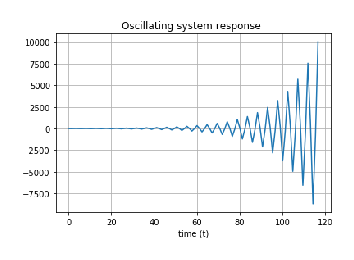
\includegraphics[width=\columnwidth]{./figs/es17btech11002/es17btech11002.eps}
\caption{}
\label{fig:es17btech11002_fig8}
\end{figure}
%
\item Find the frequency for some arbitrary R, C values given in Table \ref{table:es17btech11002_Input_Table}.\\
\begin{table}[!ht]
\centering
%%%%%%%%%%%%%%%%%%%%%%%%%%%%%%%%%%%%%%%%%%%%%%%%%%%%%%%%%%%%%%%%%%%%%%
%%                                                                  %%
%%  This is the header of a LaTeX2e file exported from Gnumeric.    %%
%%                                                                  %%
%%  This file can be compiled as it stands or included in another   %%
%%  LaTeX document. The table is based on the longtable package so  %%
%%  the longtable options (headers, footers...) can be set in the   %%
%%  preamble section below (see PRAMBLE).                           %%
%%                                                                  %%
%%  To include the file in another, the following two lines must be %%
%%  in the including file:                                          %%
%%        \def\inputGnumericTable{}                                 %%
%%  at the beginning of the file and:                               %%
%%        \input{name-of-this-file.tex}                             %%
%%  where the table is to be placed. Note also that the including   %%
%%  file must use the following packages for the table to be        %%
%%  rendered correctly:                                             %%
%%    \usepackage[latin1]{inputenc}                                 %%
%%    \usepackage{color}                                            %%
%%    \usepackage{array}                                            %%
%%    \usepackage{longtable}                                        %%
%%    \usepackage{calc}                                             %%
%%    \usepackage{multirow}                                         %%
%%    \usepackage{hhline}                                           %%
%%    \usepackage{ifthen}                                           %%
%%  optionally (for landscape tables embedded in another document): %%
%%    \usepackage{lscape}                                           %%
%%                                                                  %%
%%%%%%%%%%%%%%%%%%%%%%%%%%%%%%%%%%%%%%%%%%%%%%%%%%%%%%%%%%%%%%%%%%%%%%



%%  This section checks if we are begin input into another file or  %%
%%  the file will be compiled alone. First use a macro taken from   %%
%%  the TeXbook ex 7.7 (suggestion of Han-Wen Nienhuys).            %%
\def\ifundefined#1{\expandafter\ifx\csname#1\endcsname\relax}


%%  Check for the \def token for inputed files. If it is not        %%
%%  defined, the file will be processed as a standalone and the     %%
%%  preamble will be used.                                          %%
\ifundefined{inputGnumericTable}

%%  We must be able to close or not the document at the end.        %%
	\def\gnumericTableEnd{\end{document}}


%%%%%%%%%%%%%%%%%%%%%%%%%%%%%%%%%%%%%%%%%%%%%%%%%%%%%%%%%%%%%%%%%%%%%%
%%                                                                  %%
%%  This is the PREAMBLE. Change these values to get the right      %%
%%  paper size and other niceties.                                  %%
%%                                                                  %%
%%%%%%%%%%%%%%%%%%%%%%%%%%%%%%%%%%%%%%%%%%%%%%%%%%%%%%%%%%%%%%%%%%%%%%

	\documentclass[12pt%
			  %,landscape%
                    ]{report}
       \usepackage[latin1]{inputenc}
       \usepackage{fullpage}
       \usepackage{color}
       \usepackage{array}
       \usepackage{longtable}
       \usepackage{calc}
       \usepackage{multirow}
       \usepackage{hhline}
       \usepackage{ifthen}

	\begin{document}


%%  End of the preamble for the standalone. The next section is for %%
%%  documents which are included into other LaTeX2e files.          %%
\else

%%  We are not a stand alone document. For a regular table, we will %%
%%  have no preamble and only define the closing to mean nothing.   %%
    \def\gnumericTableEnd{}

%%  If we want landscape mode in an embedded document, comment out  %%
%%  the line above and uncomment the two below. The table will      %%
%%  begin on a new page and run in landscape mode.                  %%
%       \def\gnumericTableEnd{\end{landscape}}
%       \begin{landscape}


%%  End of the else clause for this file being \input.              %%
\fi

%%%%%%%%%%%%%%%%%%%%%%%%%%%%%%%%%%%%%%%%%%%%%%%%%%%%%%%%%%%%%%%%%%%%%%
%%                                                                  %%
%%  The rest is the gnumeric table, except for the closing          %%
%%  statement. Changes below will alter the table's appearance.     %%
%%                                                                  %%
%%%%%%%%%%%%%%%%%%%%%%%%%%%%%%%%%%%%%%%%%%%%%%%%%%%%%%%%%%%%%%%%%%%%%%

\providecommand{\gnumericmathit}[1]{#1} 
%%  Uncomment the next line if you would like your numbers to be in %%
%%  italics if they are italizised in the gnumeric table.           %%
%\renewcommand{\gnumericmathit}[1]{\mathit{#1}}
\providecommand{\gnumericPB}[1]%
{\let\gnumericTemp=\\#1\let\\=\gnumericTemp\hspace{0pt}}
 \ifundefined{gnumericTableWidthDefined}
        \newlength{\gnumericTableWidth}
        \newlength{\gnumericTableWidthComplete}
        \newlength{\gnumericMultiRowLength}
        \global\def\gnumericTableWidthDefined{}
 \fi
%% The following setting protects this code from babel shorthands.  %%
 \ifthenelse{\isundefined{\languageshorthands}}{}{\languageshorthands{english}}
%%  The default table format retains the relative column widths of  %%
%%  gnumeric. They can easily be changed to c, r or l. In that case %%
%%  you may want to comment out the next line and uncomment the one %%
%%  thereafter                                                      %%
\providecommand\gnumbox{\makebox[0pt]}
%%\providecommand\gnumbox[1][]{\makebox}

%% to adjust positions in multirow situations                       %%
\setlength{\bigstrutjot}{\jot}
\setlength{\extrarowheight}{\doublerulesep}

%%  The \setlongtables command keeps column widths the same across  %%
%%  pages. Simply comment out next line for varying column widths.  %%
\setlongtables

\setlength\gnumericTableWidth{%
	53pt+%
	93pt+%
0pt}
\def\gumericNumCols{2}
\setlength\gnumericTableWidthComplete{\gnumericTableWidth+%
         \tabcolsep*\gumericNumCols*2+\arrayrulewidth*\gumericNumCols}
\ifthenelse{\lengthtest{\gnumericTableWidthComplete > \linewidth}}%
         {\def\gnumericScale{\ratio{\linewidth-%
                        \tabcolsep*\gumericNumCols*2-%
                        \arrayrulewidth*\gumericNumCols}%
{\gnumericTableWidth}}}%
{\def\gnumericScale{1}}

%%%%%%%%%%%%%%%%%%%%%%%%%%%%%%%%%%%%%%%%%%%%%%%%%%%%%%%%%%%%%%%%%%%%%%
%%                                                                  %%
%% The following are the widths of the various columns. We are      %%
%% defining them here because then they are easier to change.       %%
%% Depending on the cell formats we may use them more than once.    %%
%%                                                                  %%
%%%%%%%%%%%%%%%%%%%%%%%%%%%%%%%%%%%%%%%%%%%%%%%%%%%%%%%%%%%%%%%%%%%%%%

\ifthenelse{\isundefined{\gnumericColA}}{\newlength{\gnumericColA}}{}\settowidth{\gnumericColA}{\begin{tabular}{@{}p{53pt*\gnumericScale}@{}}x\end{tabular}}
\ifthenelse{\isundefined{\gnumericColB}}{\newlength{\gnumericColB}}{}\settowidth{\gnumericColB}{\begin{tabular}{@{}p{93pt*\gnumericScale}@{}}x\end{tabular}}

\begin{tabular}[c]{%
	b{\gnumericColA}%
	b{\gnumericColB}%
	}

%%%%%%%%%%%%%%%%%%%%%%%%%%%%%%%%%%%%%%%%%%%%%%%%%%%%%%%%%%%%%%%%%%%%%%
%%  The longtable options. (Caption, headers... see Goosens, p.124) %%
%	\caption{The Table Caption.}             \\	%
% \hline	% Across the top of the table.
%%  The rest of these options are table rows which are placed on    %%
%%  the first, last or every page. Use \multicolumn if you want.    %%

%%  Header for the first page.                                      %%
%	\multicolumn{2}{c}{The First Header} \\ \hline 
%	\multicolumn{1}{c}{colTag}	%Column 1
%	&\multicolumn{1}{c}{colTag}	\\ \hline %Last column
%	\endfirsthead

%%  The running header definition.                                  %%
%	\hline
%	\multicolumn{2}{l}{\ldots\small\slshape continued} \\ \hline
%	\multicolumn{1}{c}{colTag}	%Column 1
%	&\multicolumn{1}{c}{colTag}	\\ \hline %Last column
%	\endhead

%%  The running footer definition.                                  %%
%	\hline
%	\multicolumn{2}{r}{\small\slshape continued\ldots} \\
%	\endfoot

%%  The ending footer definition.                                   %%
%	\multicolumn{2}{c}{That's all folks} \\ \hline 
%	\endlastfoot
%%%%%%%%%%%%%%%%%%%%%%%%%%%%%%%%%%%%%%%%%%%%%%%%%%%%%%%%%%%%%%%%%%%%%%

\hhline{|-|-}
	 \multicolumn{1}{|p{\gnumericColA}|}%
	{\gnumericPB{\centering}\gnumbox{\textbf{Parameter}}}
	&\multicolumn{1}{p{\gnumericColB}|}%
	{\gnumericPB{\centering}\gnumbox{\textbf{Value}}}
\\
\hhline{|--|}
	 \multicolumn{1}{|p{\gnumericColA}|}%
	{\gnumericPB{\centering}\gnumbox{$R$}}
	&\multicolumn{1}{p{\gnumericColB}|}%
	{$250 \Omega$}
\\
\hhline{|--|}
	 \multicolumn{1}{|p{\gnumericColA}|}%
	{\gnumericPB{\centering}\gnumbox{$C$}}
	&\multicolumn{1}{p{\gnumericColB}|}%
	{$1mF$}
\\
\hhline{|-|-|}
	 \multicolumn{1}{|p{\gnumericColA}|}%
	{\gnumericPB{\centering}\gnumbox{$R_{2}$}}
	&\multicolumn{1}{p{\gnumericColB}|}%
	{$2030\Omega $}
\\
\hhline{|--|}
	 \multicolumn{1}{|p{\gnumericColA}|}%
	{\gnumericPB{\centering}\gnumbox{$R_{1}$}}
	&\multicolumn{1}{p{\gnumericColB}|}%
	{$1000\Omega $}	
\\
\hhline{|-|-|}
\end{tabular}

\ifthenelse{\isundefined{\languageshorthands}}{}{\languageshorthands{\languagename}}
\gnumericTableEnd

\caption{}
\label{table:es17btech11002_Input_Table}
\end{table}
\\
\solution 
%
\textbf{Frequency:} From equation \eqref{eq:es17btech11002_freq}
\begin{align}
\omega = \frac{1}{RC} = 10000 rad/sec
\end{align}
\begin{align}
f = \frac{\omega }{2\pi} = 1.57 kHz
\end{align}
\item Verify the frequency using spice simulation.\\
\solution The following readme file provides necessary instructions to simulate the circuit in spice.
\begin{lstlisting}
codes/es17btech11002/spice/README
\end{lstlisting}
The following netlist simulates the given circuit.
\begin{lstlisting}
codes/es17btech11002/spice/es17btech11002.net
\end{lstlisting}
The following code plots the output from the oscillator spice simulation which is shown in Fig. \ref{fig:es17btech11002_spice}.
\begin{lstlisting}
codes/es17btech11002/spice/es17btech11002_spice.py
\end{lstlisting}
\renewcommand{\thefigure}{\theenumi.\arabic{figure}}
%
\begin{figure}[!ht]
\centering
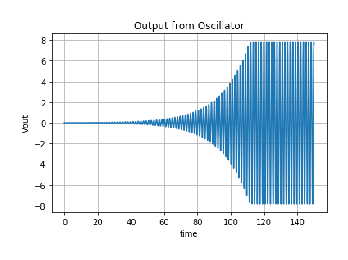
\includegraphics[width=\columnwidth]{./figs/es17btech11002/es17btech11002_spice.eps}
\caption{}
\label{fig:es17btech11002_spice}
\end{figure}
%
The following code plots a part of the spice output from which we can observe a clear sinusoidal output shown in Fig. \ref{fig:es17btech11002_spice2}.
\begin{lstlisting}
codes/es17btech11002/spice/es17btech11002_spice2.py
\end{lstlisting}
\begin{figure}[!ht]
\centering
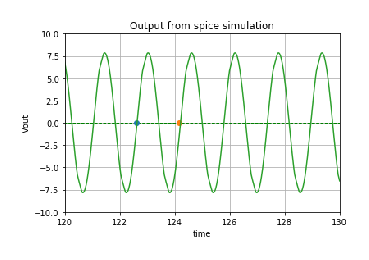
\includegraphics[width=\columnwidth]{./figs/es17btech11002/es17btech11002_spice2.eps}
\caption{}
\label{fig:es17btech11002_spice2}
\end{figure}
\renewcommand{\thefigure}{\theenumi}
\textbf{Amplitude:}From Fig. \ref{fig:es17btech11002_spice2} V(peak-peak) is 
\begin{align}
V_{p-p} &= 0.47-(-0.47) = 0.94V
\end{align}
\begin{align}
V_{max} &= \frac{V_{p-p}}{2} = 0.47.
\end{align}
\textbf{Frequency:} time period is calculated by any two end points of one cycle,
\begin{align}
T&=0.0313164 - \brak{0.03060} = 0.7164 ms
\end{align}
\begin{align}
f = \frac{1}{T} = 1.39 kHz
\end{align}
Hence,the frequency is verified through the spice simulation.
\end{enumerate}

\end{document}
